\documentclass[10pt,a4paper]{article}
\usepackage[T1]{fontenc}
\usepackage[utf8]{inputenc}
\usepackage{newtxtext,newtxmath}
\usepackage[a4paper,left=19mm,right=19mm,top=17mm,bottom=17mm,footskip=8mm]{geometry}
\usepackage{microtype,graphicx,booktabs,tabularx,multicol,array,xcolor,wrapfig}
\usepackage[font=small,labelfont=bf,skip=3pt]{caption}
\usepackage[compact,small]{titlesec}
\usepackage[hidelinks]{hyperref}
\usepackage{enumitem}
\usepackage[titles]{tocloft}
\setcounter{tocdepth}{1}
\renewcommand{\cftsecfont}{\normalfont}
\renewcommand{\cftsecpagefont}{\normalfont}
\setlength{\cftbeforesecskip}{0pt}
\renewcommand{\cftsecleader}{\cftdotfill{\cftdotsep}}
\setlist{nosep,leftmargin=1.2em,topsep=1pt,itemsep=1pt}
\setlength{\parskip}{2.5pt plus 1pt}
\setlength{\parindent}{0pt}
\titlespacing*{\section}{0pt}{7pt plus 2pt}{2pt}
\setlength{\textfloatsep}{7pt plus 2pt}
\setlength{\floatsep}{5pt plus 2pt}
\setlength{\intextsep}{5pt plus 2pt}
\newcommand{\para}[1]{\textbf{#1}\enspace}
\newcommand{\cte}[1]{[#1]}
\hypersetup{pdftitle={Does the camera model change the outcome?},pdfauthor={Nicolo Iacobone}}
\graphicspath{{../results/figures/}}

\begin{document}

\begin{center}
{\Large\bfseries Does the camera model change the outcome?\par}
\vspace{1pt}
{\large A simulated RealSense D415 on aluminium parts, for pose estimation and suction grasping\par}
\vspace{2pt}
{\small Nicolo Iacobone \quad·\quad November 2026 \quad·\quad Code and results: \href{https://github.com/NicoloIacobone/synthetic-rgbd-manufacturing-perception}{\texttt{github.com/NicoloIacobone/synthetic-rgbd-manufacturing-perception}}\par}
\end{center}
\vspace{-2pt}

\noindent\fbox{\parbox{\dimexpr\textwidth-2\fboxsep-2\fboxrule}{\small
\textbf{Summary.} I built a pipeline that generates labelled synthetic RGB-D scenes of aluminium T-slot profiles and L-brackets and simulates the active-stereo sensing chain of an Intel RealSense D415: rendered infrared stereo pairs with the projected dots, metal and matte materials at 850\,nm, sensor noise and semi-global matching. I then ran one pre-specified experiment on 460 paired instance-views (a part in a view) in 50 test scenes. CAD-based pose recall at 5\,mm is 0.717 on ideal depth, 0.561 with independent noise matched to a published D415 measurement, 0.343 with the camera model on matte parts and 0.070 on metal. All three pre-specified comparisons reject equal recall. So, in this simulation, the camera model changes the outcome and independent per-pixel noise does not stand in for it; of the 49 points between that noise and the model on metal, 27 are specific to metal. The size of the effect on a real camera remains open: metal recall rises to 0.276 on a rougher surface, and I could not source the true roughness; my primary renders have no ambient light although the imagers are unfiltered; and on real D415 images of one metal part the disparity errors are compatible, but the real camera flags 21\% of part pixels invalid against 2.3\% in the model.}}

{\small\vspace{3pt}\noindent\textbf{Contents}\vspace{-4pt}
\begin{multicols}{3}
\makeatletter\@starttoc{toc}\makeatother
\end{multicols}}
\vspace{-6pt}

\section{Problem and scope}
A robot that picks and assembles aluminium profiles and brackets needs depth on surfaces that are hard for active stereo, because smooth metal reflects the projected pattern like a mirror instead of scattering it, so the texture the matcher needs is weak or changes with the viewpoint. The D415 datasheet specifies depth on a white target and says nothing about metal \cte{1}. My question is whether modelling this camera changes the result of a downstream step, compared with ideal depth and with noise of the size the camera is known to have.
\textbf{Not in scope:} detection (ground-truth masks are given), grasp execution, a real robot, training networks, and replicating Intel's matching chip. \textbf{Results apply} to an active-stereo model with D415 geometry and to this ICP, not to a physical D415.

\section{Related work}
\para{Depth simulation.} A common route adds noise to ideal depth. Dex-Net 2.0 and 3.0 train grasp networks on rendered depth with multiplicative and Gaussian-process noise \cte{2,3}, and Dex-Net 3.0 lists objects with ``specularities or transparencies that prevent the depth camera from sensing the object geometry'' among its failure cases \cte{3}. A second route simulates the sensing process. Landau et al.\ predict Kinect infrared and depth images from the projector, dot pattern and disparity processing \cte{4}, and DepthSynth extends this idea to more structured-light sensors, reporting that the data improves recognition and pose networks \cte{5}. Two simulators target the D415 directly. Zhang et al.\ combine material acquisition, ray-traced infrared rendering, infrared noise and semi-global matching, and report perception and control policies that transfer to a real robot without fine-tuning; they also note that their specular, translucent and transparent real objects, unlike their matte 3D-printed ones, give ``noisy and incomplete'' depth, ``more challenging to simulate'' \cte{6}. DREDS renders in Blender, randomises materials from specular to diffuse, and trains a depth-restoration network that raised real grasp success on specular and transparent objects from 38.8\% to 96.2\% (49 and 26 attempts) \cte{7}.

\para{Reflective industrial parts.} T-LESS provides thirty texture-less, industry-relevant objects \cte{8}. ROBI gives D415 and Ensenso images of seven metal parts, with ground truth from anti-reflective spray, and reports ``significant degradation'' of D415 depth accuracy against the Ensenso \cte{9}. XYZ-IBD, a preprint, records 15 metallic parts with three sensors including a D415 at 600--1000\,mm, and reports a ``stark performance degradation'' of current pose methods compared with household benchmarks \cte{10}. On general objects the BOP challenges point the other way: synthetic training has become competitive \cte{11,12}.

\para{What this report adds.} The studies above mostly evaluate networks trained on simulated depth, where training data, architecture and sensor model are mixed together. I use an untrained CAD-based harness, so depth is the only variable. On metal parts I compare the camera model with noise at a level measured on the real camera on a plane, with paired statistics over scenes. The price is that the result belongs to this ICP and says nothing about transfer to reality.

\section{Reference camera}
I chose the D415 for four reasons. It is an active infrared stereo camera, so material-dependent errors can emerge from rendering instead of being hand-written. It has an independent metrology study \cte{13}. It has real recordings on metal parts with ground truth \cte{9}. And it is still listed as a current product \cte{14}. For a real cell, a structured-light industrial sensor such as the Ensenso in ROBI, which outperforms the D415 there \cte{9}, would be the natural first choice; without hardware, what decided was having real D415 data on metal to check the model against. The geometry comes from the datasheet (Rev 017) \cte{1}: baseline 55\,mm; 1280$\times$720; imager field of view 71°$\pm$1° $\times$ 44°$\pm$1° with no optical filter (pp.\,43, 71); static 850\,nm projector, 67°$\times$41° (p.\,71; p.\,45 gives 64°); minimum range 450\,mm (p.\,91). The focal length follows from the imager field, $f_x = 640/\tan 35.5^\circ = 897.25$\,px. Depth accuracy is specified as $\pm$2\% within 2\,m, on a white target at 150\,mW with auto exposure (pp.\,92--93).

\section{Synthetic data pipeline}
\begin{figure}[t]
\centering
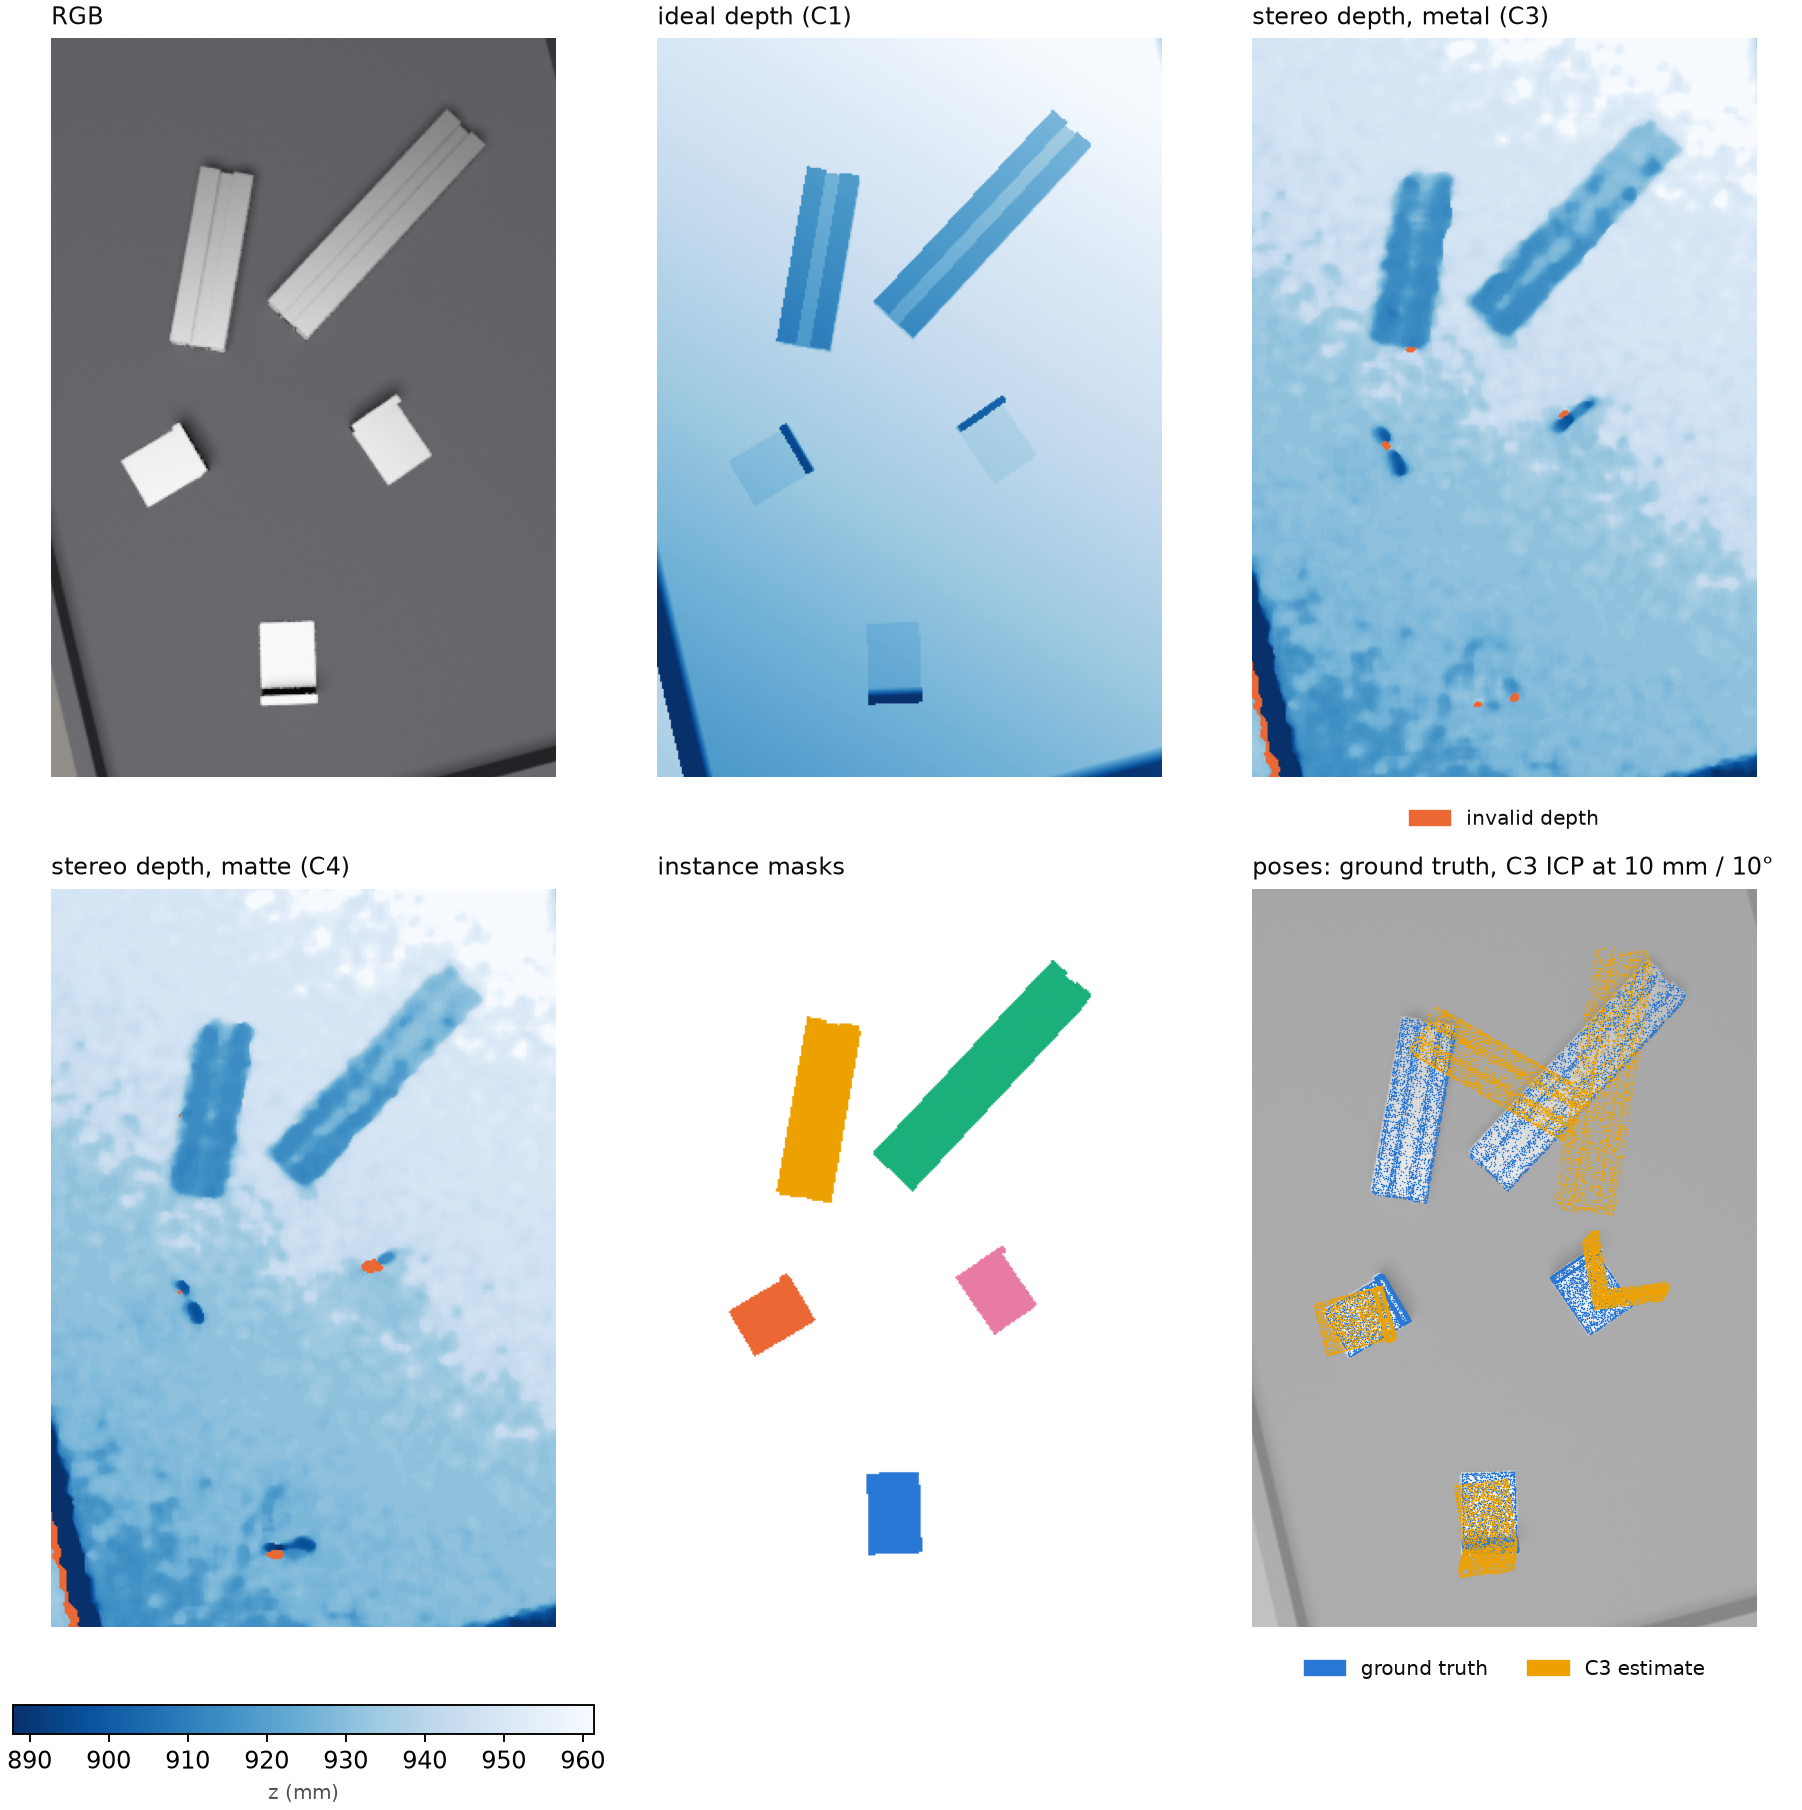
\includegraphics[width=\textwidth]{examples.png}
\caption{One test view, chosen by a rule on part types only. On metal the flat bracket at the bottom almost disappears into the tray, and ICP ends far from the true poses.}
\label{fig:examples}
\end{figure}
\para{Parts and scenes.} Parts are procedural: square T-slot-like profiles (side 30\,mm, slot opening 8\,mm, lengths 60, 100, 150\,mm) and an L-bracket (legs 40\,mm, width 30\,mm, thickness 4\,mm), with known symmetries. They are loosely based on 30-series extrusions, not on a vendor drawing. BlenderProc \cte{15} and Cycles render a tray with 3--6 parts dropped by Bullet physics, seen from two views at 0.65--0.95\,m with tilt up to 30°. I use 50 test scenes (seeds 0--49) and 5 separate development scenes (seeds 1000--1004), which never enter a confirmatory result; they serve tuning and the mechanism analysis (Fig.~\ref{fig:mechanism}). A \emph{view} is one camera image (100 on the test scenes); an \emph{instance-view} is one part in one view.

\para{Labels.} Each view is written in BOP format: RGB, ideal z-depth, visible and full masks, 6D poses, intrinsics and CAD models (Fig.~\ref{fig:examples}). Two checks guard the labels: masked depth back-projected through the labelled pose lies on the CAD surface on all 460 instance-views (worst median 0.045\,mm, no point beyond 1\,mm), and rendered depth on a tilted plane matches the analytic plane within 0.002\,mm, with the camera matrix returned within $10^{-6}$\,px.

\para{Cost.} On an 8\,GB Apple M2 a scene with all passes takes a median of 178\,s; the 50 scenes take 2\,h\,28\,min and 1.4\,GB, and the whole experiment 9\,h\,38. \texttt{scripts/setup.sh} installs from a lock file and runs 116 tests, and \texttt{scripts/quick\_run.py} reproduces one scene's numbers without Blender in about 2 minutes (tested in a clean clone on macOS, and in a Linux container).

\section{Camera model}
The model follows the sensing chain, so effects emerge rather than being painted on.
\begin{enumerate}
\item \textbf{Projector.} A point spot light at the baseline midpoint casts a fixed semi-random pattern of 30\,000 Gaussian dots ($\sigma=0.7$\,px). The D415's pattern is not published. This density puts a dot on 3.76\% of lit pixels, inside the 1--10\% that Intel's guidance calls near-ideal \cte{16}.
\item \textbf{Materials at 850\,nm.} Metal is GGX with normal reflectance 0.868, computed from aluminium's optical constants at 848\,nm \cte{17}, roughness 0.15 from fits to a measured aluminium BRDF in visible light \cte{18} (Blender's roughness $r$; Cycles 4.2 uses GGX width $\alpha=r^2$, and the fits give $\alpha=0.016$--$0.022$, i.e.\ $r=0.13$--$0.15$; I use the rough end), and a 1.5\% diffuse lobe from the same fits. Matte parts are Lambertian, albedo 0.25, set on the development scenes so that mean exposed brightness on part pixels equals that of metal (16.0\,DN each). On the test scenes the match is only approximate: 15.1\,DN against 20.9\,DN on average, with a per-view ratio from 0.09 to 4.35.
\item \textbf{Light transport.} Cycles path tracing with 32 samples, 3 glossy bounces and no denoiser. Both images are rendered 128\,px wider, so the invalid left band comes from geometry and not from OpenCV's fixed margin. Linear radiance is stored, so exposure is applied later.
\item \textbf{Sensor.} A per-frame gain brings the mean of the metal left image to 20\,DN (digital numbers, the 8-bit grey levels); the same gain applies to the right image and to the matte pass. Noise is shot plus read, $\mathrm{DN}+\sqrt{\mathrm{DN}/e+\sigma_r^2}\,n$, with $n$ standard normal, an effective $e=0.42$ electrons per DN, $\sigma_r=1$\,DN and draws shared by metal and matte. Images are then quantised to 8 bits, as in the D415's streams (p.\,81).
\item \textbf{Matching.} OpenCV SGBM \cte{19}, single-pass mode, with a 7$\times$7 block, smoothness penalties $P_1$, $P_2$ of 8 and 32 times the block area, uniqueness 10, left-right check 1, speckle filter 100\,px. The search is 128\,px with disparities above 126 masked, the D415's range from \cte{13,22}. No hole filling; invalid depth stays invalid.
\end{enumerate}
\begin{table}[t]
\centering\footnotesize
\caption{Effects included and left out, and why.}\label{tab:effects}
\vspace{-1pt}
\begin{tabularx}{\textwidth}{@{}p{0.285\textwidth}X@{}}
\toprule
\textbf{Included} & \textbf{How it arises} \\
\midrule
Depth noise growing with $z^2$ & Disparity error through $z=fB/d$ \cte{20} \\
Invalid left band, occlusion shadows & Stereo and projector geometry; band within about 1\,px of $B f/z$ \\
Minimum range & 126\,px search; simulated transition at 392\,mm, see Section~\ref{sec:fail} \\
Edge fattening, flying pixels & Matching window: in the matte condition 29.1\% of edge pixels and 11.1\% of interior pixels are off by more than 5\,mm \\
Subpixel locking & SGBM's estimator. Comparable in size to the D4 chip at default firmware \cte{21}; a different mechanism \\
Glints, dark faces, reflected dots, dependence on incidence angle & GGX and 3 glossy bounces in Cycles \\
Auto exposure, shot and read noise, 8 bits & Applied to linear radiance. A mean-brightness target is assumed; Intel's algorithm is not published \\
Unlit image margins & 67° projector inside a 71° imager: 13.6\% of the image, 0.064\% of part pixels \\
\midrule
\textbf{Left out} & \textbf{Why} \\
\midrule
Ambient light, visible and infrared & The imagers have no optical filter \cte{1}, so room light reaches them; the primary run is a dark cell. My one test (Table~\ref{tab:moves}) leans towards harm: on untextured parts, ambient light can only lower dot contrast, not reveal surface texture \\
Motion blur, rolling shutter & The scene is static at capture \\
Intel's matcher and post-processing & Proprietary; raw depth only. SGBM is cross-checked on real images (Section~\ref{sec:results}) \\
Calibration error, lens distortion, thermal drift & Assumed calibrated out, with constant temperature \\
Laser speckle, projector hot spot & Intel calls speckle ``very detrimental'' and its figure shows a hot spot \cte{16}; no source quantifies them for the D415, and the datasheet is silent \\
Temporal noise & Single-frame setting \\
Anodising, machining marks, surface oxide & No source for extruded profiles at 850\,nm; only roughness is varied (Table~\ref{tab:moves}) \\
RGB imperfections & Neither task reads RGB. It is rendered from the left imager's viewpoint with a placeholder material, not modelled on the D415's RGB sensor \\
\bottomrule
\end{tabularx}
\end{table}

\para{Plane check.} On a matte plane at 0.5--1.0\,m with noise and auto exposure, bias stays within 0.31\% of $z$, the central 80\% of the image is 100\% valid, and the left band is within 1.2\,px of $B f/z$. Plane-fit RMS is 0.42--2.66\,mm, non-monotonic because of subpixel locking, the pull of estimated disparities towards whole pixels. For comparison the formula with $\varepsilon_d=0.08$\,px and my $f$ gives 1.62\,mm at 1\,m \cte{20,22}, Carfagni et al.\ measured a standard deviation of 4.74\,mm from a reference plane at 1\,m \cte{13}, and the datasheet allows 2\% of range. \textbf{This check is not independent:} $e$ is set to bring the central-region RMS to 0.09\,px, inside Intel's 0.07--0.11\,px \cte{16} (measured: 0.0897\,px). It also says nothing about metal.

\section{Experiment}
\para{Conditions,} on identical scenes and poses. \textbf{C1} ideal depth. \textbf{C2a} and \textbf{C2b} ideal depth plus Gaussian noise $\sigma=z^2\varepsilon_d/(fB)$ \cte{20}, the naive baseline: $\varepsilon_d=0.08$\,px from Intel's guide \cte{22}, and $\varepsilon_d=0.234$\,px fitted to Carfagni's 4.74\,mm at 1\,m \cte{13}, deliberately high: it is noisier than my model on the simulated plane (at most 2.66\,mm), which makes the comparison with C3 conservative. \textbf{C3} the camera model on metal. \textbf{C4} the camera model on matte parts, with brightness matched on the development scenes. C3 against C4 therefore contrasts the material, but brightness still differs from view to view on test scenes. \textbf{Expected:} C1 $>$ C3; C2b $>$ C3, the main claim, that noise of the size measured on a real plane overestimates recall on metal; and C4 $>$ C3.

\para{Task A, pose (primary).} Ground-truth masks, eroded by 2\,px, select depth points. Point-to-plane ICP \cte{23} aligns them to 200\,000 CAD samples with CAD normals, ray-cast visibility and coarse-to-fine stages. It starts 10\,mm and 10° from the true pose, in random directions shared across conditions. Error is MSSD \cte{11}, which handles symmetries. \textbf{The primary endpoint is recall at MSSD $<$ 5\,mm.} The 5\,mm threshold is my own, not sourced. Starts of 2, 5 and 20\,mm and degrees are secondary.

\para{Task B, suction.} On the masked points, the planner takes the flattest point that fits a 10\,mm-radius cup. Success is checked on the true mesh: within 2\,mm of the surface, normal within 15°, and the whole disk planar within 1\,mm on one part. With this cup no profile face can pass (largest flat disk: radius 9.76\,mm), so I report brackets separately.

\para{Statistics and pre-specification.} The unit is a part in a view: 460 instance-views (342 profiles, 118 brackets), none excluded by the 10\% visibility rule of BOP \cte{11}. Endpoint, thresholds, conditions and the test/development split were frozen under a git tag before any data existed; the fixed sequence and C2b's level were added after the tag but before any test data were rendered. Tests run in a fixed sequence at $\alpha=0.05$, C1 vs C3, then C2b vs C3, then C3 vs C4. A comparison rejects only if the exact two-sided McNemar $p<0.05$ and the 95\% scene-bootstrap interval (10\,000 resamples of whole scenes) excludes zero. McNemar treats instance-views as independent, although they cluster in views and scenes, so its $p$ values are too small; the scene bootstrap carries the clustering. Settings were fixed by rules declared in advance, each looking at one allowed statistic: sensor noise on a simulated plane, exposure and albedo on development scenes, material constants from sources. Camera settings never saw recall. The ICP variant was chosen on development recall, by its worst case across conditions and, on ties, the next worst. As a bug detector, ICP on C1 started at the true pose must keep at least 99\% of instance-views below 0.5\,mm; it keeps 460/460.

\para{Deviations I must disclose.} Two matter most; all are logged with reasons in \texttt{docs/PLAN.md}. (i) The sanity check first failed on the test scenes because of a bug (Section~\ref{sec:fail}). The fix changed the harness after the test render; only C1 at zero offset had been seen. (ii) \textbf{After all results had been seen}, a datasheet check showed that I had derived $f_x$ from the 65° depth field, while the datasheet's formulas use the 71° imager field. I re-rendered and re-ran everything. The new run is primary whatever its direction, and it is the one reported here. Exposure, matte albedo and both noise levels that depend on $f$ were re-derived by the same rules; material, matcher and harness were not touched. The 65° results appear only as a sensitivity (Table~\ref{tab:results}), and they were not used to choose settings.

\section{Results}\label{sec:results}
\begin{table}[t]
\centering\footnotesize
\caption{Results on 460 instance-views (commit \texttt{7eca5f0}, clean tree; 95\% intervals over scenes). Below the line: descriptive passes, outside the tests. Last column: the archived run with the earlier focal length, a sensitivity only.}\label{tab:results}
\vspace{-1pt}
\begin{tabular}{@{}lccccccc@{}}
\toprule
 & \multicolumn{3}{c}{Recall, MSSD $<$ 5\,mm} & Recall & Median & Suction, & Recall \\
\cmidrule(lr){2-4}
Condition & all parts & profiles & brackets & $<$ 2\,mm & MSSD, mm & brackets & at 65° \\
\midrule
C1 ideal depth & 0.717 (0.671--0.761) & 0.696 & 0.780 & 0.546 & 1.6 & 0.771 & 0.732 \\
C2a noise 0.08\,px & 0.735 (0.684--0.783) & 0.737 & 0.729 & 0.446 & 2.5 & 0.737 & 0.749 \\
C2b noise 0.234\,px & 0.561 (0.498--0.621) & 0.635 & 0.347 & 0.154 & 4.3 & 0.534 & 0.590 \\
\textbf{C3 metal, camera model} & \textbf{0.070} (0.046--0.095) & 0.079 & 0.042 & 0.000 & 16.8 & 0.110 & 0.085 \\
C4 matte, camera model & 0.343 (0.287--0.400) & 0.380 & 0.237 & 0.059 & 7.3 & 0.381 & 0.386 \\
\midrule
Metal, roughness 0.2 & 0.139 (0.100--0.180) & 0.167 & 0.059 & 0.007 & 12.4 & 0.136 & 0.159 \\
Metal, roughness 0.4 & 0.276 (0.218--0.335) & 0.345 & 0.076 & 0.033 & 9.4 & 0.229 & 0.288 \\
Metal, reflections off & 0.076 (0.054--0.100) & 0.088 & 0.042 & 0.004 & 17.3 & 0.161 & 0.102 \\
Matte, albedo 0.5 & 0.363 (0.302--0.427) & 0.401 & 0.254 & 0.063 & 6.8 & 0.373 & 0.444 \\
\bottomrule
\end{tabular}
\end{table}
\begin{figure}[t]
\centering
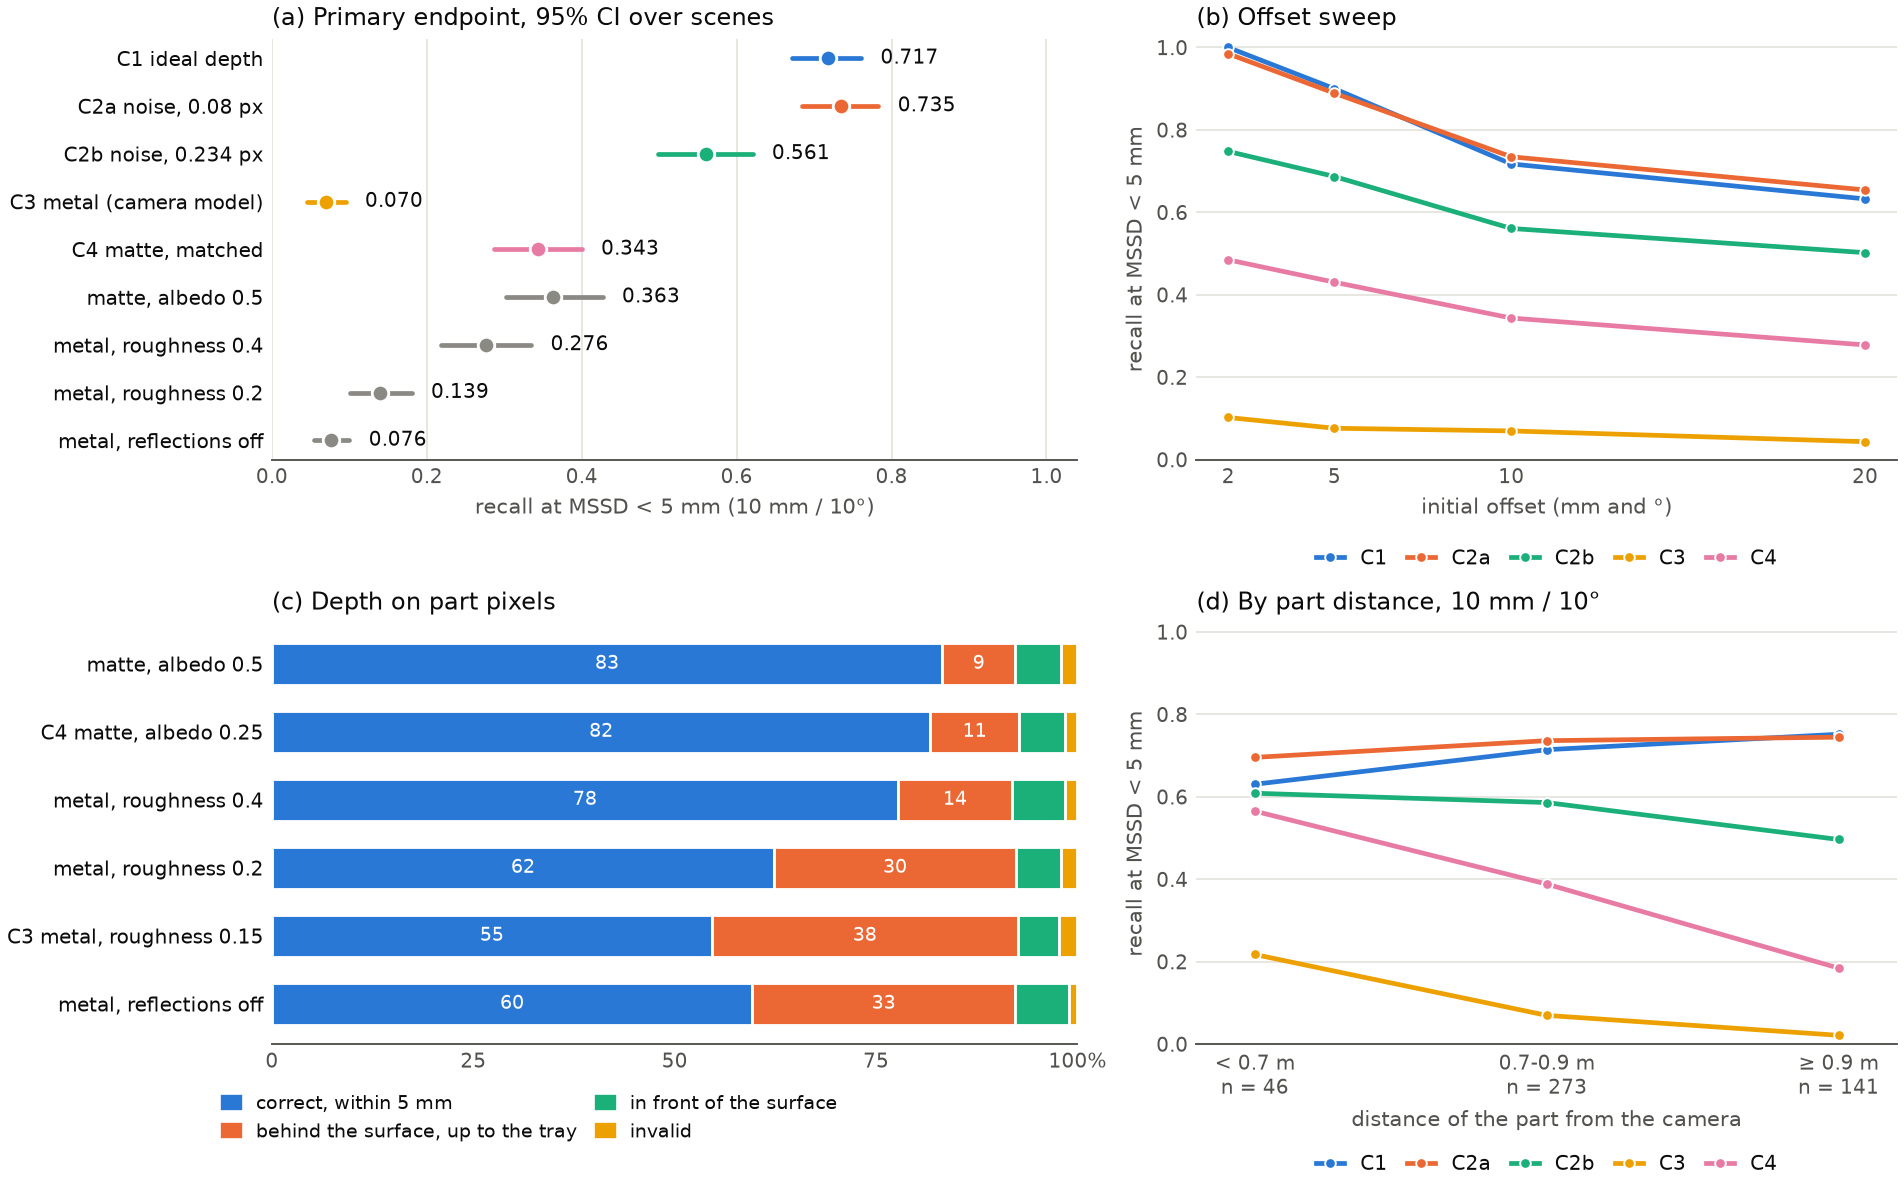
\includegraphics[width=0.9\textwidth]{results.png}
\caption{(a) Primary endpoint, with 95\% scene-bootstrap intervals (460 instance-views, 50 scenes). (b) Recall by starting offset. (c) Depth on part pixels. (d) Recall by part distance, at 10\,mm / 10°.}
\label{fig:results}
\end{figure}
\para{Confirmatory result.} All three comparisons reject equal recall, in percentage points: C1$-$C3 +64.8 (59.6 to 70.0), C2b$-$C3 +49.1 (42.5 to 55.9) and C3$-$C4 $-$27.4 ($-$33.0 to $-$21.7), with McNemar $p<10^{-29}$ in all three, unadjusted for clustering. Even if each scene counted as a single paired observation, the smallest effects detectable at 80\% power (33.2, 29.3, 22.2 points) would be smaller than those observed. The order \{C1, C2a\} $>$ C2b $>$ C4 $>$ C3 holds at all four offsets. So, in this simulation, \textbf{the camera model changes the outcome in a way that plane-calibrated noise does not predict}: that noise gives recall a factor of eight above the model at my assumed roughness and a factor of two at roughness 0.4 (0.561 against 0.070 and 0.276), and I do not know the real value.

\para{Metal fails silently.} Only 2.3\% of metal-part pixels are invalid, yet 44.1\% of the valid ones are off by more than 5\,mm (Fig.~\ref{fig:results}c). The error is one-sided: median +3.0\,mm, 5th and 95th percentiles $-$5.2 and +29.2\,mm, against a symmetric $\pm$5.3\,mm for C2b. C3's level is not a convergence limit. From a 2\,mm / 2° start, where every instance-view already has MSSD below 5\,mm (largest 4.70\,mm), C1 keeps 1.00 and C3 ends at 0.102, so ICP on C3 moves away from the truth. C1's own fall to 0.717 at 10\,mm / 10° is a harness limit, so absolute recall belongs to this ICP, and the gaps between conditions are shown for this ICP only.

\para{Size and layout matter; the sign has no detectable effect.} I had assumed that ICP averages out zero-mean noise and fails on a one-sided bias, so I tested it on seeds 0--9, keeping each part's own errors and changing their structure, with the reading written down before the run (Table~\ref{tab:moves}). Random signs make the errors zero-mean and independent but leave the large ones where they are: recall stays at 0.102. Permuting them among the part's pixels keeps the bias and spreads the large ones: 0.255. Both together give 0.276, no different from permuting alone (+2.0 points, $-$7.8 to +11.6). \textbf{So my assumption was wrong.} Most of the drop from C1 (0.704 on these seeds) comes from the size of the errors on metal, 44.1\% of valid pixels beyond 5\,mm against 11.2\% in C2b, and the rest from their layout; my reading is that clustered errors leave whole faces without usable points. A plane measurement shows neither. With ten scenes these are indications, not estimates.

\para{Stereo alone costs more than noise, in this model.} C4 sits 21.7 points below C2b (17.5 to 26.1; descriptive) on matte parts. So of the 49.1 points between C2b and C3, 21.7 appear on matte parts too and 27.4 are specific to metal. Brightness does not explain the metal share: on test scenes metal is, if anything, brighter (20.9 against 15.1\,DN), and doubling the matte albedo moves C4 by only +2.0 points. Part of the matte gap may come from how my images look rather than from stereo as such: they are bright dots on black, unlike real ones (see ``Against real images''). No dot density I tried closes the gap: at 60\,000 dots, on seeds 0--9, C4 still sits 24.5 points below C2b (16.0 to 34.3). C2a does not differ detectably from C1: $-$1.7 points ($-$4.1 to +0.7). Noise helps profiles (16 instance-views gained, 2 lost, $p=0.001$) and may hurt brackets (2 gained, 8 lost, $p=0.11$); I did not trace why.

\para{Distance matters.} From below 0.7\,m (46 instance-views) to 0.9\,m and beyond (141 instance-views), C3 falls from 0.217 to 0.021 and C4 from 0.565 to 0.184, while C1 rises from 0.630 to 0.752. A fixed 5\,mm shrinks in disparity: 0.305\,px at 0.9\,m.

\para{Suction} (descriptive) follows the same order on the 118 bracket instance-views: C1 0.771 (0.673--0.864), C2a 0.737 (0.648--0.822), C2b 0.534 (0.436--0.635), C4 0.381 (0.280--0.484), C3 0.110 (0.046--0.178), with C1$-$C3 at +66.1 points (56.6 to 76.3). C3 plans a grasp on 44.1\% of them and 25.0\% of those succeed, against 85.6\% and 90.1\% for C1. Profiles never succeed, by geometry, yet the planner proposes a grasp on 0.3\% of profile instance-views in C1, 45.6\% in C2a, 97.1\% in C2b, 97.7\% in C4 and 93.9\% in C3. On a robot those would be false grasps, and they follow any depth error, not only the camera model's; I did not trace the mechanism.

\begin{table}[t]
\centering\footnotesize
\caption{What moves recall at 5\,mm (descriptive, same scenes and offsets). Rows below the line use seeds 0--9 and read against their own baseline.}\label{tab:moves}
\vspace{-1pt}
\begin{tabularx}{\textwidth}{@{}p{0.33\textwidth}ccX@{}}
\toprule
Change & Metal & Matte & Reading \\
\midrule
Baseline, 50 scenes & 0.070 & 0.343 & \\
Roughness 0.15 $\to$ 0.2 $\to$ 0.4 & 0.139, 0.276 & & The largest lever, and the value is not sourced for real extrusions \\
Reflections off, same material & 0.076 & & $-$0.7 points ($-$2.7 to +1.5), though correct pixels go 55 $\to$ 60\% \\
Brighter matte, albedo 0.5 & & 0.363 & +2.0 points ($-$2.0 to +5.8): darkness is not the limit \\
Two new noise draws & 0.061, 0.063 & & Spread 0.9 points; the primary draw is the highest of the three \\
ICP run again on identical depth & 0.070 & 0.343 & No instance-view crosses 5\,mm in 1840 comparisons (C1, C2b, C3, C4) \\
\midrule
Baseline, seeds 0--9 & 0.102 & 0.265 & \\
Less noise, $e$ 0.42 $\to$ 1.0 & 0.102 & 0.286 & Noise at 21\,DN 7.1 $\to$ 4.7\,DN does not explain metal \\
All three matcher filters off & 0.112 & 0.245 & No order flips; filters remove mostly wrong pixels \\
Ambient light added & 0.031 & 0.224 & Reaches 22\,DN on metal, but metal gets worse; level and spectrum not sourced \\
Each part's errors, random signs & 0.102 & & +0.0 points ($-$5.3 to +4.7): zero mean, large errors stay in place \\
Each part's errors, permuted & 0.255 & & +15.3 points (+2.2 to +32.7): bias kept, large errors spread \\
Permuted, with random signs & 0.276 & & +17.3 points (+6.7 to +28.6): the best per-part additive noise \\
Same 30\,000 dots, rendered again & 0.102 & 0.265 & No instance-view crosses 5\,mm; the next two rows read against this \\
10\,000 dots, new render & 0.041 & 0.184 & Metal $-$6.1 points ($-$11.5 to $-$1.0), matte $-$8.2 ($-$20.8 to +4.5) \\
60\,000 dots, new render & 0.031 & 0.235 & Metal $-$7.1 points ($-$12.0 to $-$2.9), matte $-$3.1 ($-$9.8 to +4.3) \\
\bottomrule
\end{tabularx}
\end{table}

\begin{figure}[t]
\centering
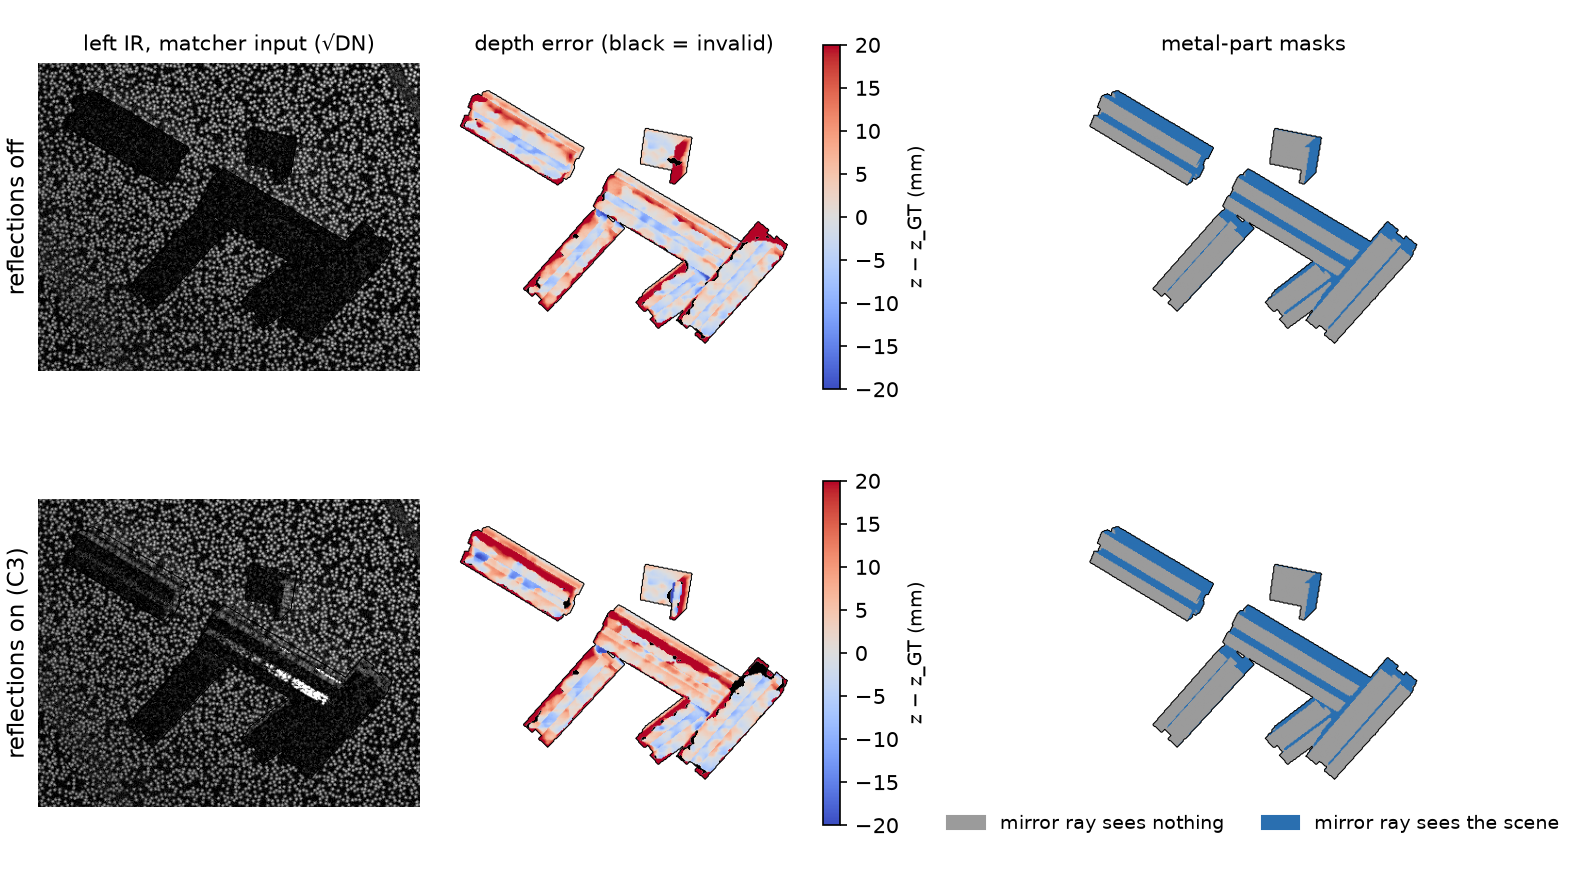
\includegraphics[width=0.7\textwidth]{mechanism.png}
\vspace{-2pt}
\caption{One development view, chosen by part-pixel count. Reflections add glints without changing the error pattern much.}
\label{fig:mechanism}
\end{figure}
\para{Mechanism: partly understood (Fig.~\ref{fig:mechanism}).} On 10 development views I did not isolate one cause. With metal blanked in both images, 98.7\% of part pixels stay valid and only 2.5\% are correct, so the matcher fills instead of invalidating. Faces whose mirror ray hits the scene are 35.7\% correct, others 56.1\%. When I shift the background of the right image by $\pm$3\,px, biased pixels do not follow it (slope 0.00), while with metal blanked the fill does (blanked control 0.77--0.94), so they are not simply copied from the tray; 86.1\% lie between surface and tray. Low texture does not explain it: pixels with no texture above noise fell from 53.5\% at 65° to 3.2\% here, with lower noise, while correct pixels stayed near 50\% (49.1, 50.5).

\begin{figure}[t]
\centering
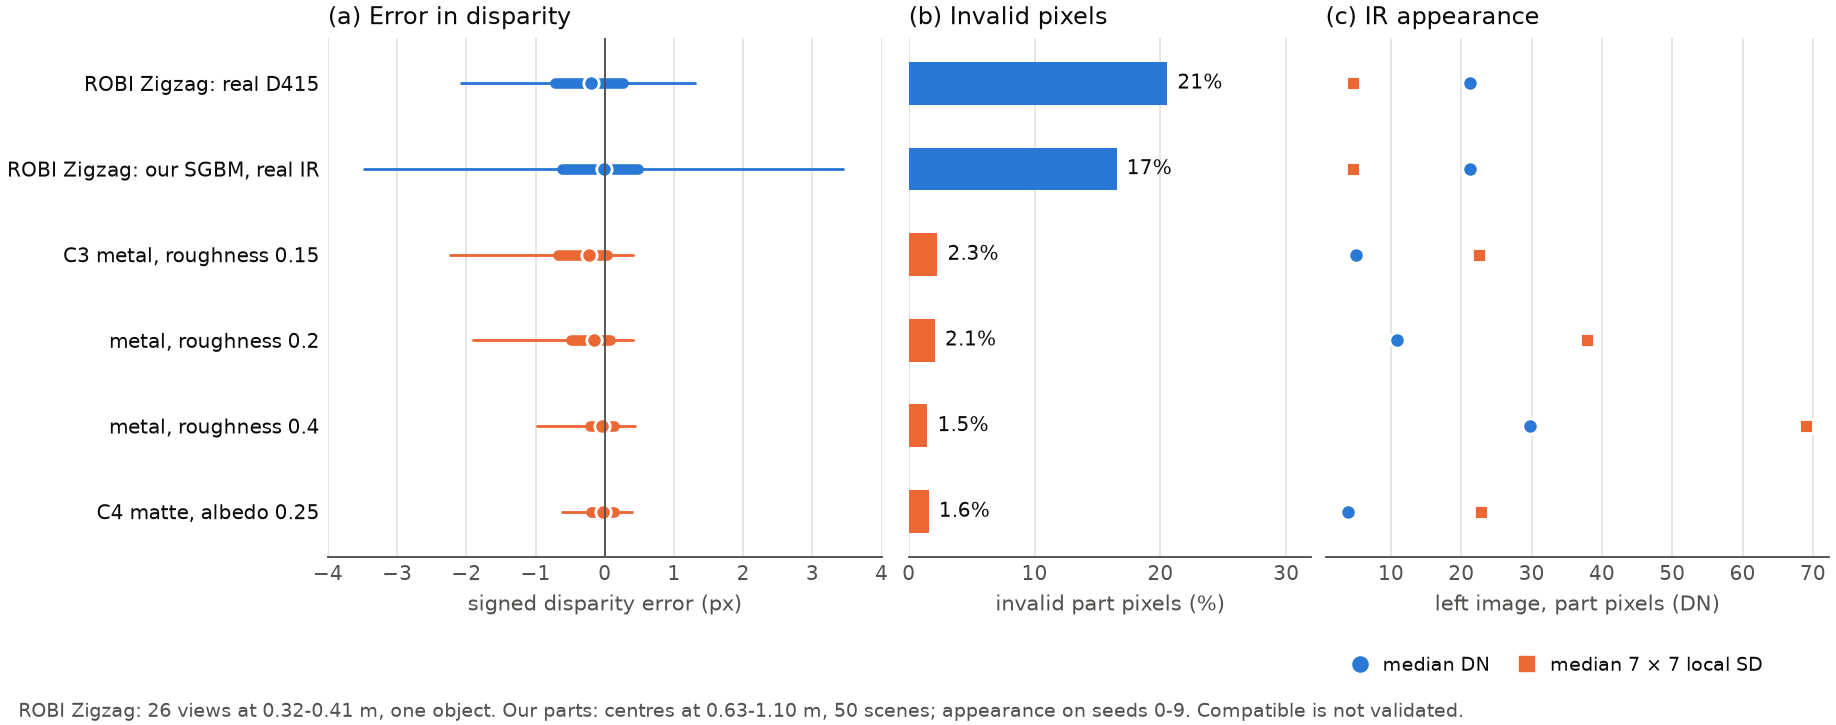
\includegraphics[width=0.9\textwidth]{robi.png}
\vspace{-2pt}
\caption{Against real D415 data on one ROBI object \cte{9}, 26 views at 0.32--0.41\,m, while my part centres lie at 0.63--1.10\,m; appearance on seeds 0--9. In pixels, since 5\,mm is 2.15\,px at 0.34\,m and 0.305\,px at 0.9\,m. Boxes: p5, p25, p50, p75, p95. Close on signed disparity error, not on invalid share or appearance: compatible, not validated.}
\label{fig:robi}
\end{figure}
\para{Against real images (Fig.~\ref{fig:robi}).} I compared with 26 ROBI Zigzag views at 0.32--0.41\,m, one object at a different range from my parts (0.63--1.10\,m). ROBI records with a disparity shift of 78\,px, so both the D4 chip and my SGBM, run on the same pairs, search 78--204\,px (about 0.24--0.64\,m), and the Zigzag parts lie well inside. Signed disparity error is close: p5, p25, p50 are $-$2.07, $-$0.71, $-$0.19\,px for the real D415 and $-$2.24, $-$0.68, $-$0.23\,px for C3, while roughness 0.4 gives $-$0.98, $-$0.22, $-$0.04\,px. But a pose-annotation error of 1\,mm would shift disparity by 0.37\,px at this range, more than the gaps between these quantiles, and ROBI states no annotation error, only a mean residual of 0.8\,mm when fitting its RealSense camera poses \cte{9}. Invalid pixels differ: 21\% real, 2.3\% in C3. SGBM on the real infrared pairs leaves 17\% invalid, so the gap comes from the images and not from my matcher (inference). Those images differ too: 21\,DN median and 4.6\,DN local contrast on real parts, against 5\,DN and 22.5\,DN in C3. The background differs as well: 21\,DN and 2.7\,DN on ROBI, against 3\,DN and 25.7\,DN here, and my matte parts look like my metal ones (4\,DN, 22.8\,DN). Materials differ, but I infer that my whole image is bright dots on black, most likely because my primary renders have no ambient light while the real, unfiltered imagers see the room; this may add to the cost of stereo in both C3 and C4. So the disparity match may be partly a coincidence. I read this as compatible, not validated.

\section{What did not work}\label{sec:fail}
\begin{itemize}
\item \textbf{Wrong focal length for most of the project.} See the deviations above. The correction also opened a mismatch I could not close: with the 126\,px search the depth transition falls at 392\,mm, against the datasheet's 450\,mm. Evidence is mixed, since 450\,mm with 126\,px would imply $f\approx1031$\,px and Intel's tuning guide computes with 65° \cte{22}, while ROBI's real camera has 905.9\,px. No scene pixel is that close.
\item \textbf{Sanity check failed.} First result 416/459 (in the run at the earlier focal length, which had 459 instance-views) against the required 99\%. Cause: a bug in AI-written code, where a ray-cast cache gave profiles the mesh of another length, culling end faces the camera sees. Development data (40 instance-views) and 94 unit tests had missed it. After the fix and denser CAD sampling all variants pass. I chose the sample count after seeing C1 at zero offset on test scenes, which I disclose.
\item \textbf{No reflections in the first renders.} BlenderProc defaults to zero glossy bounces, so early metal had no reflected dots. A figure checked before the test render exposed it, and every dependent setting was re-derived.
\item \textbf{A cup that fits no profile.} The 10\,mm-radius cup was frozen in the protocol. Only later, but before any suction data, did I find that no profile face can hold it (largest flat disk: radius 9.76\,mm), so suction is informative only for brackets and I report part types separately. The planner still proposes grasps on 46--98\% of profile instance-views under every depth error tested, against 0.3\% on ideal depth.
\item \textbf{A robustness check that did nothing.} In OpenCV 5.0.0, \texttt{disp12MaxDiff}\,=\,$-$1 does not disable the left-right check. The first robustness run therefore left it on. I re-ran it with the check really off, and a unit test now pins this behaviour.
\item \textbf{Fragile noise calibration.} The same rule gave $e=0.087$ at 65° and 0.42 at 71°, because locking alone sets a no-noise floor (0.053, then 0.075\,px) close to the 0.09\,px target. The value is effective, not physical.
\item \textbf{Not repeatable.} Renders with identical settings differ slightly, and in one development view 79\% of metal pixels moved by more than 5\,mm. A repeat render of seeds 0--9 was gentler: it changed 0.14\% of metal depth pixels in the median view and moved no instance-view across 5\,mm. ICP on bit-identical depth also varies on unstable instance-views, with a source I did not trace. I measured what this costs: a full repeat of C1, C2b, C3 and C4 moved at most 6 of 460 instance-views by more than 0.01\,mm per condition (the largest by 33\,mm), but no instance-view crossed 5\,mm, so recall is identical and the three tests reject again.
\item \textbf{A depth overflow found in the final review.} Depth is stored as uint16 at 0.1\,mm, so a match beyond 6.55\,m (disparity below 7.5\,px) wraps around to a false depth, as low as 26\,mm. It touches 0.09\% of image pixels but none of the 1\,674\,189 part pixels in C3 and C4, so recall and part metrics do not change. With all filters off (Table~\ref{tab:moves}) it touches 0.04\% of part pixels on seeds 0--9. I documented it rather than change the depth code just before submission.
\item \textbf{Predictions I got wrong.} I expected the left-band check to fail at 71° because of the unlit margin, but the matcher fills that strip with plausible depth, itself an artefact. I expected texture loss to explain metal, and then a one-sided pull; neither does.
\item \textbf{Not done:} global registration without an initial pose, parallel-jaw grasping, noise redraws on matte.
\end{itemize}

\section{Limitations}
Masks are ground truth, and real masks would degrade at edges. Scenes are sparse trays, not dense bins or mated assemblies, whose concave metal corners would add inter-reflections, and the parts carry no surface texture such as die lines. The ICP variant was chosen on development data by a margin of one instance-view. Part of C1's shortfall is likely geometric, as the protocol anticipated: ICP can slide along a profile's axis unless an end face is visible. Absolute recall therefore reflects how observable the parts are, and I claim only differences between conditions under the same harness. SGBM is not Intel's matcher, though on real ROBI pairs at close range it comes near the D4 chip (70\% against 71\% of pixels within 5\,mm, invalid 17\% against 21\%). Roughness rests on a visible-light fit to an aluminium sample of unstated finish; I expect, without a source, anodised profiles to be more diffuse, which would make 0.070 pessimistic. Most importantly, the primary run is a dark cell seen by unfiltered imagers: room light would add passive texture on real parts and highlights of the lamps on metal, so C3, C4 and the invalid share could move either way. The dot density is also assumed, because the pattern is not published. On seeds 0--9 metal recall falls with both fewer and more dots, from 0.102 to 0.041 and 0.031 (Table~\ref{tab:moves}), so the metal level depends on the pattern. Changing the count also moves every dot, so I cannot separate density from layout, and my 30\,000 dots may be a favourable draw. The order C3 $<$ C4 $<$ C2b holds at all three densities. At 60\,000 dots the images are still far from real ones: background 11\,DN, local contrast 16.4\,DN, against 21\,DN and 2.7\,DN on ROBI. Infrared images use 32 samples: on one development scene at the earlier focal length, 128 samples moved correct pixels by 1.95 points (my limit was 2), but lit-metal radiance differed by a median of 47--53\%, so the images are not converged. Render noise is thus an error on metal with no physical counterpart: it does not move recall (a repeat render of seeds 0--9 moved no instance-view across 5\,mm), but it is part of every pixel-level statistic on metal, including the mechanism analysis and the comparison with ROBI. Parts are procedural. Detectable effects are about 7--10 points on 50 scenes and larger on ten, so small differences among descriptive rows mean little. Above all, nothing here was measured on a real profile.

\section{Reflection: the riskiest assumption}
\para{The assumption.\footnote{Sections 10 and 11 together are the one-page answer to the assignment's last question: about 0.87 of a page, across a page break.}} \emph{That the simulated sensor errs in the same way as the real one, on the parts that matter.} Appearance gets most of the attention in sim-to-real work, and there the evidence is encouraging: in BOP 2022 a pose method trained only on BlenderProc images reached 82.7 ARC (BOP's average-recall score), and the gap to methods also trained on real images shrank \cte{12}. Depth on reflective metal is a different problem, for three reasons that come out of this work.
\begin{itemize}
\item \textbf{The error is not what a plane measurement suggests.} Noise at a level measured on the real camera predicts 0.561 where the camera model predicts 0.070. Part of the gap is size: on metal 44\% of valid pixels are off by more than 5\,mm, against 11\% with that noise. Part is layout: independent noise of the model's own sizes still gives 0.276 against 0.102 on the same ten scenes. None of this shows on the flat white target on which cameras are specified. A network trained on the wrong errors would learn the wrong correction.
\item \textbf{Even the kind of failure is uncertain.} In my model only 2.3\% of metal pixels are flagged invalid while 44\% of the rest are off by more than 5\,mm, and nothing in the depth map shows which. On the only real D415 data I could compare, the camera flags 21\% invalid instead. Two plausible error models thus predict different failures, a silent bias or visible holes, and a network trained on one would meet the other. Validation in simulation cannot tell them apart, because the same model produces the training and the test data; the first evidence comes from the robot.
\item \textbf{Nothing I could find pins it down.} Metal recall moved nearly fourfold across roughness values, I found no source for extruded profiles at 850\,nm, and my renders omit the room light that the unfiltered imagers see. XYZ-IBD reports stark degradation on metal parts in cluttered bins \cte{10}, and Zhang et al.\ note that specular and transparent real objects are harder to simulate than matte 3D-printed ones \cte{6}.
\end{itemize}
Two other candidates are real but show themselves sooner: appearance randomisation that misses factory surfaces \cte{24} fails visibly in the first real images, and pose error that does not predict pick success appears in the first trials. A wrong sensor error model can stay hidden until grasps fail on one surface finish at one distance. More generally, for any perception model trained mainly on synthetic data, the simulator's error model for the deployed sensor on the deployed materials is the assumption that validation in simulation cannot check.

\section{The first six months}
The aim is to measure this gap on real parts, then decide from evidence how much sensor realism is worth.
\begin{itemize}
\item \textbf{Month 1, no hardware.} Repeat my comparison on the D415 depth of XYZ-IBD \cte{10}, which is at my working range (600--1000\,mm) and covers 15 metal objects, unlike the single ROBI object at 0.32--0.41\,m used here. Extend the ROBI comparison to its other six objects, whose infrared pairs let me separate the images from the matcher. Run two cheap tests on my own data: a stronger additive baseline (spatially correlated noise with dropout at the real invalid share), and marking the wrong metal pixels invalid, to measure what silent failure costs compared with holes.
\item \textbf{Months 1--2, calibration set.} Record real extruded profiles and brackets, mill-finish and anodised, 20--30 scenes at 0.6--1.0\,m, with a D415 and a structured-light reference on a robot arm for repeatable views. Take ground truth from anti-reflective spray, as ROBI and XYZ-IBD do. Depth and both infrared streams together are supported only for calibration (datasheet p.\,84), so record them in succession.
\item \textbf{Months 2--3, measure effect by effect.} Build a digital twin of the same poses. Compare infrared appearance first, then invalid share and signed disparity error, by material, incidence angle and distance. Add the cell's own lighting, visible and infrared, with a measured spectrum, since the imagers are unfiltered.
\item \textbf{Months 3--4, fix by evidence.} Measure the BRDF of the real parts at 850\,nm instead of assuming roughness. Learn a residual only for what physics leaves over, and randomise only what stays unmodelled, within measured bounds. Hold out one part family and one finish. \textbf{Gate, fixed in advance:} on held-out scenes, invalid share within 5 points and disparity quantiles within 0.25\,px of real (5\,mm is 0.305\,px at 0.9\,m). If it fails, the model stays labelled as unvalidated.
\item \textbf{Months 5--6, does it matter?} Train one pose and one suction network on ideal depth, naive noise, the fitted model and randomised depth, then test all four on real parts in closed-loop pick and assembly, with thresholds and a minimum useful gain declared in advance. If the fitted model does not beat naive noise by that margin, effort should go elsewhere, and that is a result worth publishing.
\end{itemize}
\para{Outputs:} an open real-and-simulated dataset on aluminium parts, a validated sensor model with stated limits, and a measured answer to how much sensor realism a factory perception model needs. Compared with \cte{6,7}, the parts are aluminium extrusions in their real finishes at working range, and the model is judged against a gate fixed in advance. If hardware access slips, months 1--3 run on XYZ-IBD and ROBI alone, and the closed-loop test shrinks to suction on brackets.

\section{AI-use note}
I used Claude Code (Claude Opus 5.5) as planning partner, literature searcher and programmer: it wrote most of the code, ran the experiments, and produced the first draft of this report from the project's records. I took the decisions, set the rules for what could be tuned on what, and checked the results and this text. Among my decisions: an untrained harness so that depth is the only variable, making the comparison with real ROBI data mandatory, and the dot-density and ambient-light tests. A second AI session, acting as a sceptical reviewer, read the final draft; its points were checked against the data, and two that did not hold were dropped. A log of corrections is in \texttt{docs/AI\_USE\_LOG.md}.
\textbf{Where I disagreed:} when the assistant found the focal-length error, it recommended disclosing it as a limitation without re-rendering, because the estimated effect was small and the value was frozen. I rejected that and had the render and the whole experiment re-run as a logged deviation. \textbf{Where checking mattered:} when the sanity check failed, the assistant's first explanation (numerical conditioning) did not hold; the diagnosis I asked for, why fitness was low on ideal depth, confirmed the real cause, a bug in its own cache code. My rule that every source be checked against the primary text also caught errors in its earlier citations.

{\footnotesize
\section*{References}
\vspace{-3pt}
\begin{multicols}{2}
\setlength{\parskip}{0.6pt}
\begin{enumerate}[leftmargin=1.7em,label={[\arabic*]},itemsep=0.4pt,topsep=0pt]
\item Intel. RealSense D400 Series Product Family Datasheet, Rev 017, doc.\ 337029-017, Sep 2023.
\item Mahler et al. Dex-Net 2.0: Deep learning to plan robust grasps with synthetic point clouds and analytic grasp metrics. RSS 2017.
\item Mahler et al. Dex-Net 3.0: Computing robust vacuum suction grasp targets in point clouds using a new analytic model and deep learning. ICRA 2018.
\item Landau, Choo, Beling. Simulating Kinect infrared and depth images. IEEE Trans.\ Cybernetics 46(12), 2016.
\item Planche et al. DepthSynth: Real-time realistic synthetic data generation from CAD models for 2.5D recognition. 3DV 2017.
\item Zhang et al. Close the optical sensing domain gap by physics-grounded active stereo sensor simulation. IEEE Trans.\ Robotics 39(3), 2023.
\item Dai et al. Domain randomization-enhanced depth simulation and restoration for perceiving and grasping specular and transparent objects. ECCV 2022.
\item Hodaň et al. T-LESS: An RGB-D dataset for 6D pose estimation of texture-less objects. WACV 2017.
\item Yang et al. ROBI: A multi-view dataset for reflective objects in robotic bin-picking. IROS 2021.
\item Huang et al. XYZ-IBD: Benchmarking robust 6D object pose estimation under real-world industrial complexity. arXiv:2506.00599v3, 2026.
\item Hodaň et al. BOP Challenge 2020 on 6D object localization. ECCV Workshops 2020.
\item Sundermeyer et al. BOP Challenge 2022 on detection, segmentation and pose estimation of specific rigid objects. arXiv:2302.13075, 2023.
\item Carfagni et al. Metrological and critical characterization of the Intel D415 stereo depth camera. Sensors 19(3):489, 2019.
\item RealSense. Products page, realsenseai.com/products, and spin-out notice (Intel Capital, Jul 2025).
\item Denninger et al. BlenderProc2: A procedural pipeline for photorealistic rendering. JOSS 8(82):4901, 2023.
\item Grunnet-Jepsen et al. Projectors for Intel RealSense depth cameras D4xx. Intel white paper, Rev 1.0, 2019.
\item Rakić et al. Optical properties of metallic films for vertical-cavity optoelectronic devices. Appl.\ Opt.\ 37, 1998.
\item Bieron, Peers. An adaptive BRDF fitting metric. Computer Graphics Forum 39(4), 2020, and GGX supplement.
\item Hirschmüller. Stereo processing by semiglobal matching and mutual information. IEEE TPAMI 30(2), 2008; OpenCV \texttt{StereoSGBM} implements a modified version.
\item Keselman et al. Intel RealSense stereoscopic depth cameras. CVPR Workshops 2017.
\item Grunnet-Jepsen et al. Subpixel linearity improvement for Intel RealSense depth camera D400 series. Intel white paper, Rev 1.3, 2019.
\item Grunnet-Jepsen et al. Best-known-methods for tuning Intel RealSense D400 depth cameras for best performance. Intel white paper, Rev 2.0.
\item Rusinkiewicz, Levoy. Efficient variants of the ICP algorithm. 3DIM 2001.
\item Tobin et al. Domain randomization for transferring deep neural networks from simulation to the real world. IROS 2017.
\end{enumerate}
\end{multicols}
}
\end{document}
